\subsection{Problem 4}

\textbf{The definition of a pairing heap does not state which elements are neighbors. For the solution of the next tasks we assume a sorted list of roots (by insertion order) and neighborhood induced by this. Given is a Pairing Heap in the following state.}

\begin{enumerate}
    \item \textbf{Give a very short sequence of operations that creates this state.}
    
    insert(0) \\
    insert(1) \\
    insert(2) \\
    insert(3) \\
    insert(4) \\
    insert(5) \\
    insert(6) \\
    deleteMin() \\
    insert(0) \\
    deleteMin() \\
    insert(0) \\
    deleteMin() \\
    insert(8) 
    
    \item \textbf{Execute the following operations step by step on the given heap and draw the intermediate state of the heap after each operation: deleteMin(), insert(9), decreaseKey(a,1), remove(b).}

    \begin{center}
        \makebox[\textwidth]{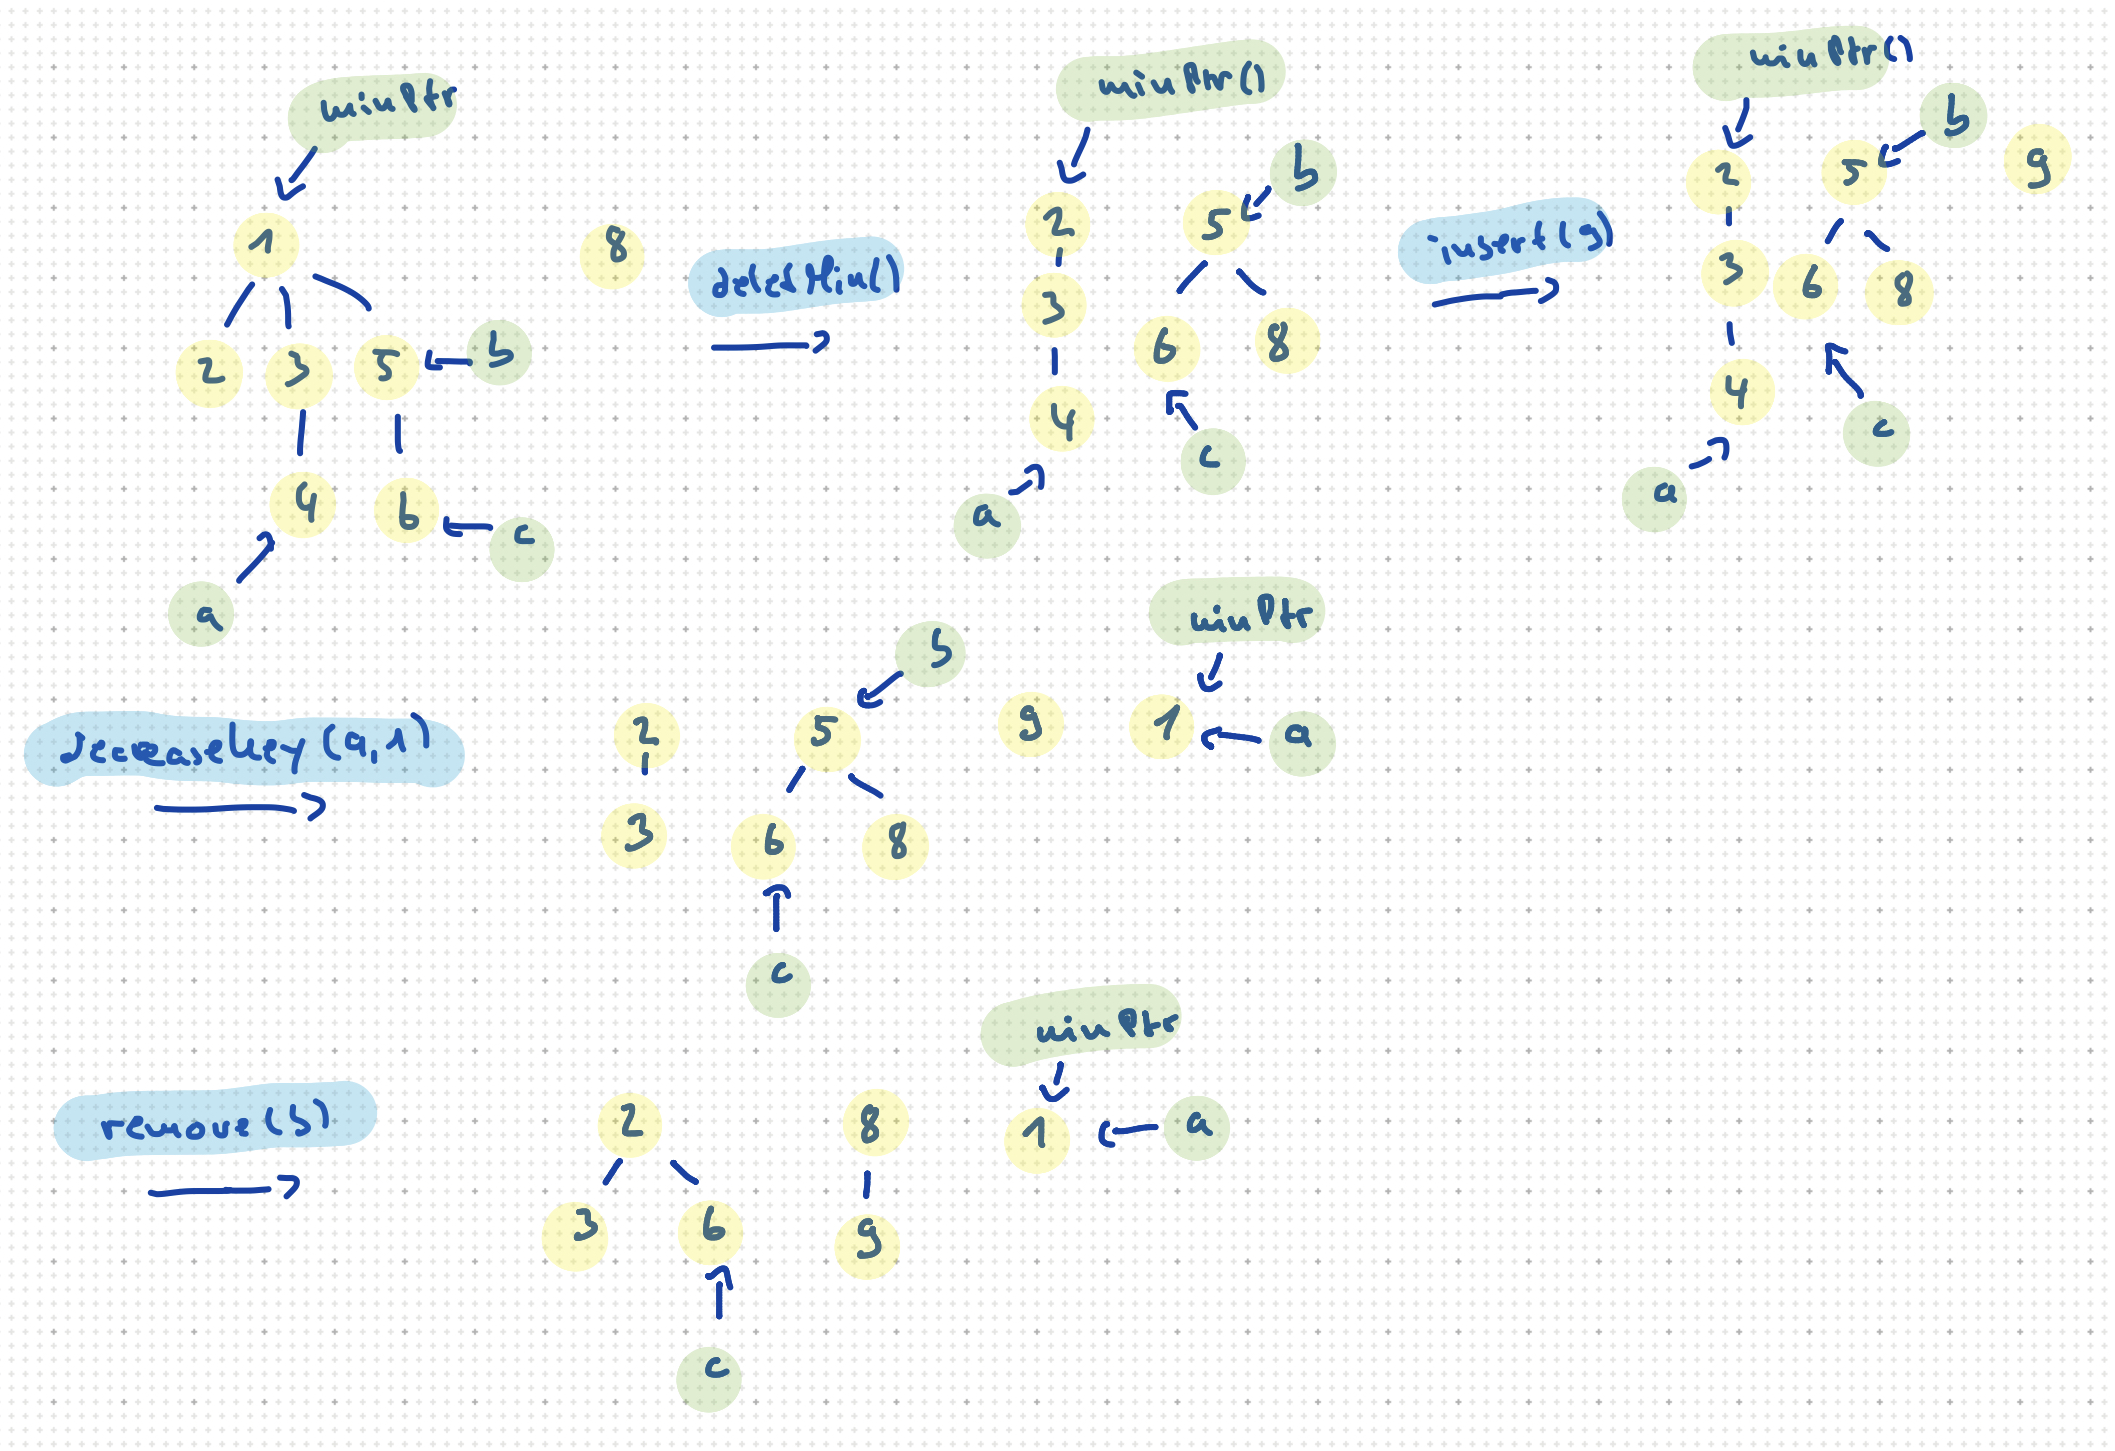
\includegraphics[width=\textwidth]{images/exercise_4.jpeg}}
    \end{center}

\end{enumerate}